The previous chapter looked at persistent memory programming from the perspective of consistency models and programming interface.
While necessary to define correct program behavior, I did not consider actual implementations or what optimizations provide optimal performance.
This chapter considers two simple persistent programming patterns -- a persistent log/buffer and a persistent linked list.
While I will describe how the persistent memory consistency models of the previous chapters operate with each, the point is to highlight potential performance bottlenecks and necessary optimizations.
I do not yet consider actual programming models or hardware to provide these optimizations.

Prior work has examined building data structures for NVRAM \fixme{cite BFPS, Shivaram, IBM log, NVRAM structures for analytics}.
However, these works generally address other issues such as write endurance, suggest data structures that semantically fit NVRAM without concern for performance \fixme{Shivaram}, or propose complicated software mechanisms to work around incomplete or inferior persistent consistency models \fixme{IBM}.
While \fixme{BPFS} takes a more holistic approach, their model falls short in terms of correctness, multi-threaded performance, and I believe certain single threaded-workloads, as I will show shortly.

\section{Performance}
\label{sec:PMC_patterns:Performance}

In the previous chapter I made a number of statements regarding the performance of NVRAM without much explanation.
Here I describe how I expect NVRAM, the memory system, and the programming model to affect performance.
Later sections will use these assumptions to reason about data structure performance and imaging performance optimizations.

There are primarily two cases where persists may cause a thread to stall: ordering barriers and sync barriers.
Ordering barriers may operate by stalling at the barrier until all previous persists complete, obviously stalling the thread of execution.
More complex memory systems (such as BPFS) allow threads to continue executing ahead of persistent state, using a buffer to store persists (either in the cache or a memory buffer).
If these buffers become full threads will need to stall until room becomes available.
Therefore, persist throughput is the primary concern -- buffers allow threads to execute ahead of persistent state, but the average rate of persist must match the average rate of execution, otherwise stalls necessarily occur.

Persist throughput is primarily limited by the number of persist dependencies in an applications.
Memories typically allow high throughput so long as reads and writes may occur in parallel.
Persist dependencies reduce parallelism, requiring that some set of writes persist entirely before any dependent persists begin.
Since NVRAM cells may take up to microseconds to persists the longest dependence chain of persists may easily limit execution throughput and cause stalls.
Persistent memory consistency models stand to improve throughput and reduce stalls by relaxing persist ordering constraints and minimize the persist critical path.
The ultimate goal is to reduce persist critical path sufficiently that persist throughput exceeds execution throughput, providing the throughput of a DRAM system with the persistence of NVRAM.

Persistent memory applications also introduce stalls at sync barriers.
These are barriers used when interacting with the outside world (e.g., displaying something on-screen, communicating over the network).
Unless this external communication can be ordered with persists, allowing the thread to continue doing other useful work, the thread must stall for previous persists to complete, hurting throughput.
Additionally, end-to-end latency is important for many applications and tasks -- greater sync time (while persists drain/flush) leads to increased task latency.
Again, persist critical path determines sync latency; if all independent writes may persist in parallel the time to sync is determined by the longest chain of persists outstanding at the time sync is called.

The remainder of this chapter looks at two simple data structures, reasoning about durability while at the same time considering the persist critical path.
While some of the problems highlighted here can be circumvented by software techniques (e.g., only allowing a single thread to persist, using control flow to conditionally place epoch boundaries), this misses the point of persistent memory consistency -- to provide an easily programmable interface.
Rather, I assume the most straightforward and intuitive software design, investigating memory system optimizations.
However, I do not consider actual implementations.

\section{Persistent Buffer}
\label{sec:PMC_patterns:Buffer}

\begin{figure}
\centering
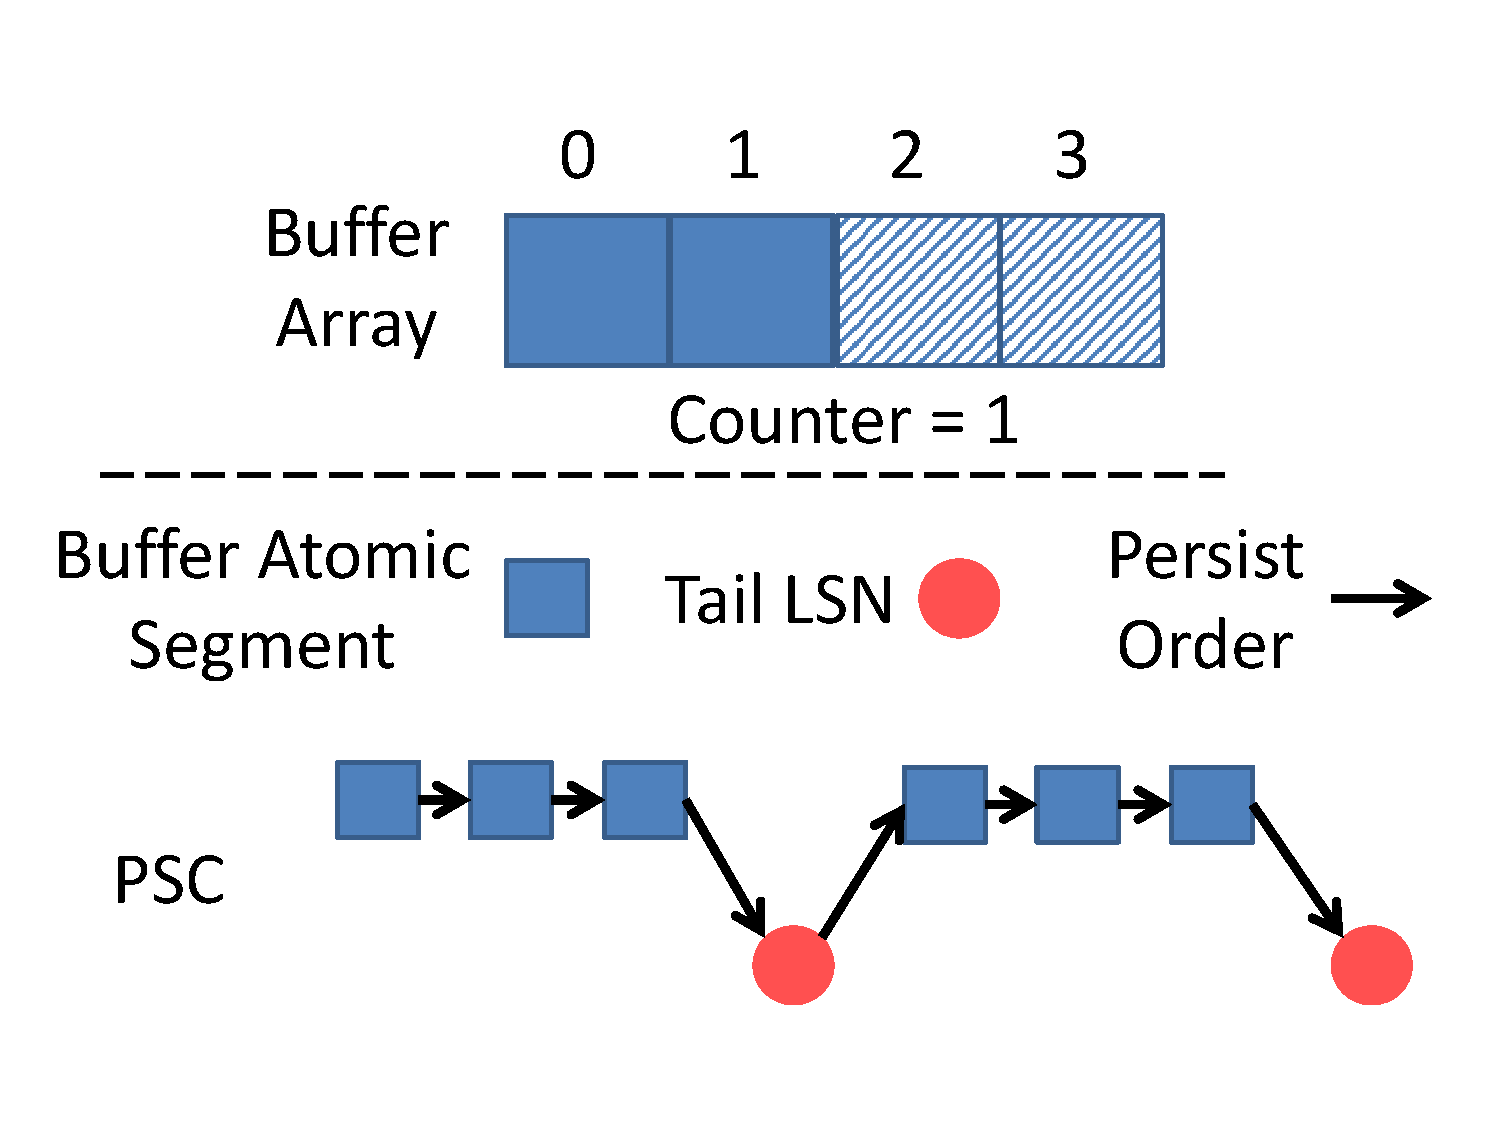
\includegraphics[width=\textwidth]{PMC_patterns/buffer.pdf}
\caption{Persistent buffer. The persistent buffer constists of a persistent array and counter (top).  The array holds persistent data.  The persistent counter marks the greatest persistent slot.  Persisting to the buffer under PSC places depdencies between writing buffer data and updating the counter, as well between persisting the counter and the next buffer persist, forming a chain (bottom).  This occurs both for single threaded and multithreaded use.}
\label{fig:buffer}
\end{figure}

\begin{figure}
\centering
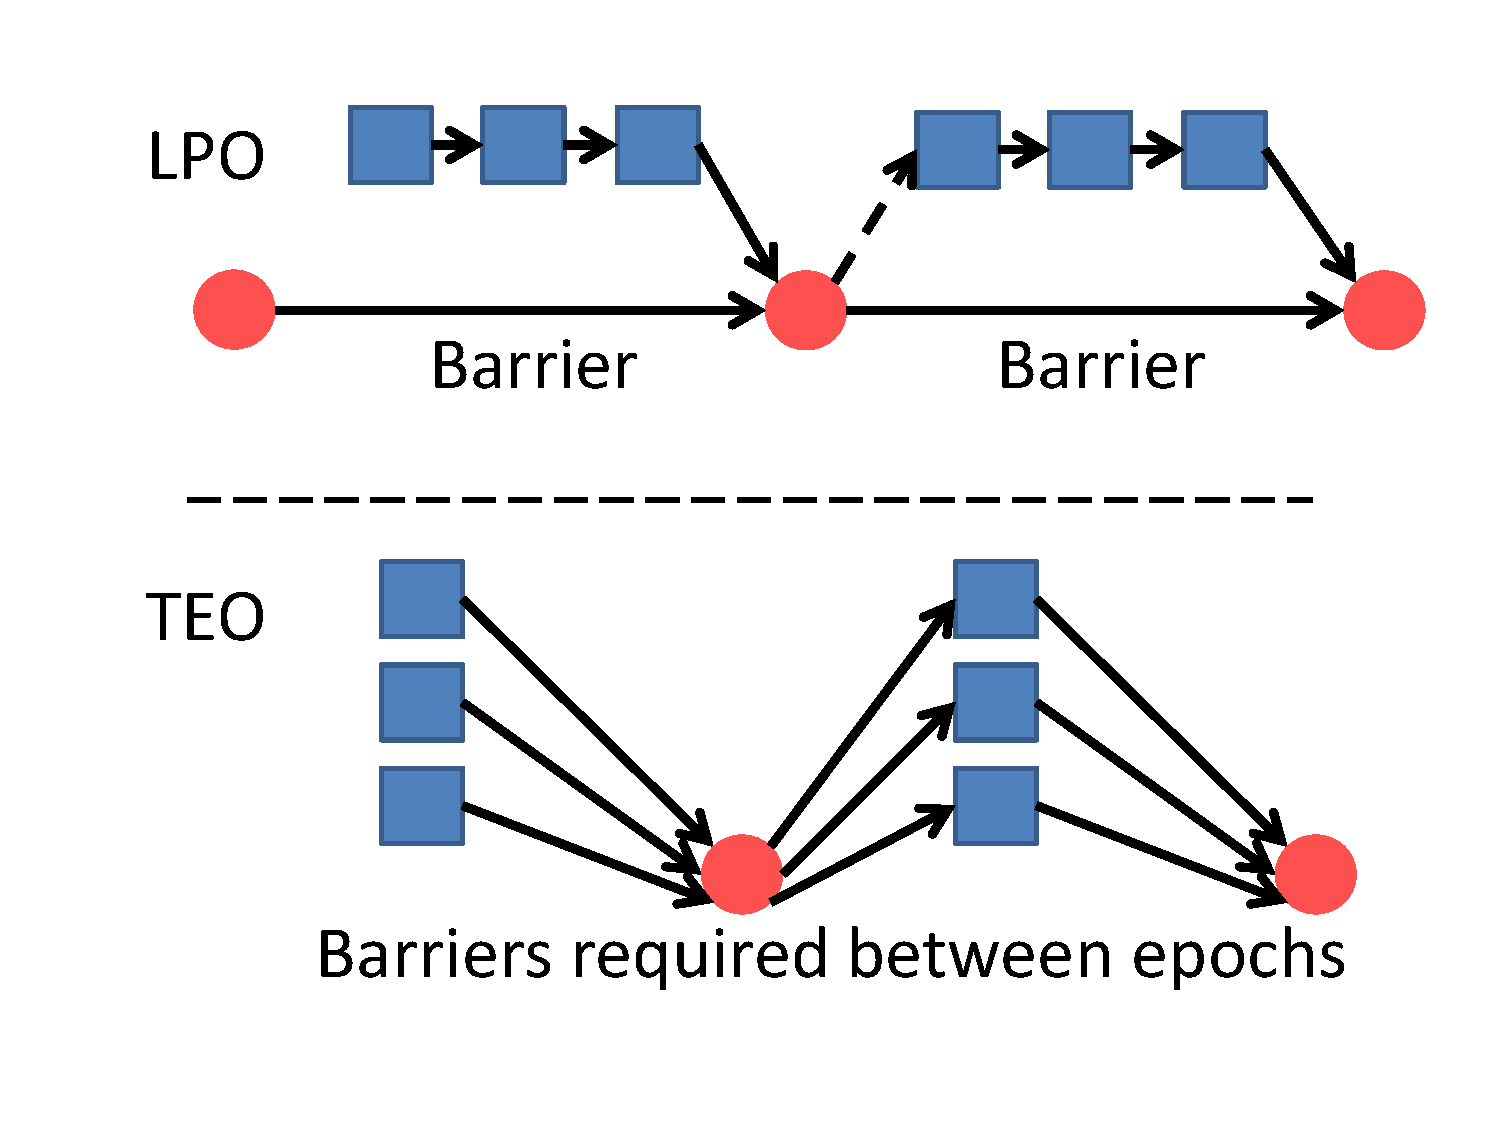
\includegraphics[width=\textwidth]{PMC_patterns/buffer_TEO_LPO.pdf}
\caption{Buffer execution under LPO and TEO.  LPO (top) removes persist dependencies between persisting the counter value and subsequent buffer persists.  Such dependencies still remain when adjacent buffer inserts are from the same thread.  Atomic persist segments within each buffer persist serialize.  TEO (bottom) allows buffer data to persist in parallel.  Buffer data necessarily persists before counter data for correctness, but counter values additionally persist before subsequent buffer persists, even from remote threads.}
\label{figure::buffer_TEO_LPO}
\end{figure}

\begin{figure}
\centering
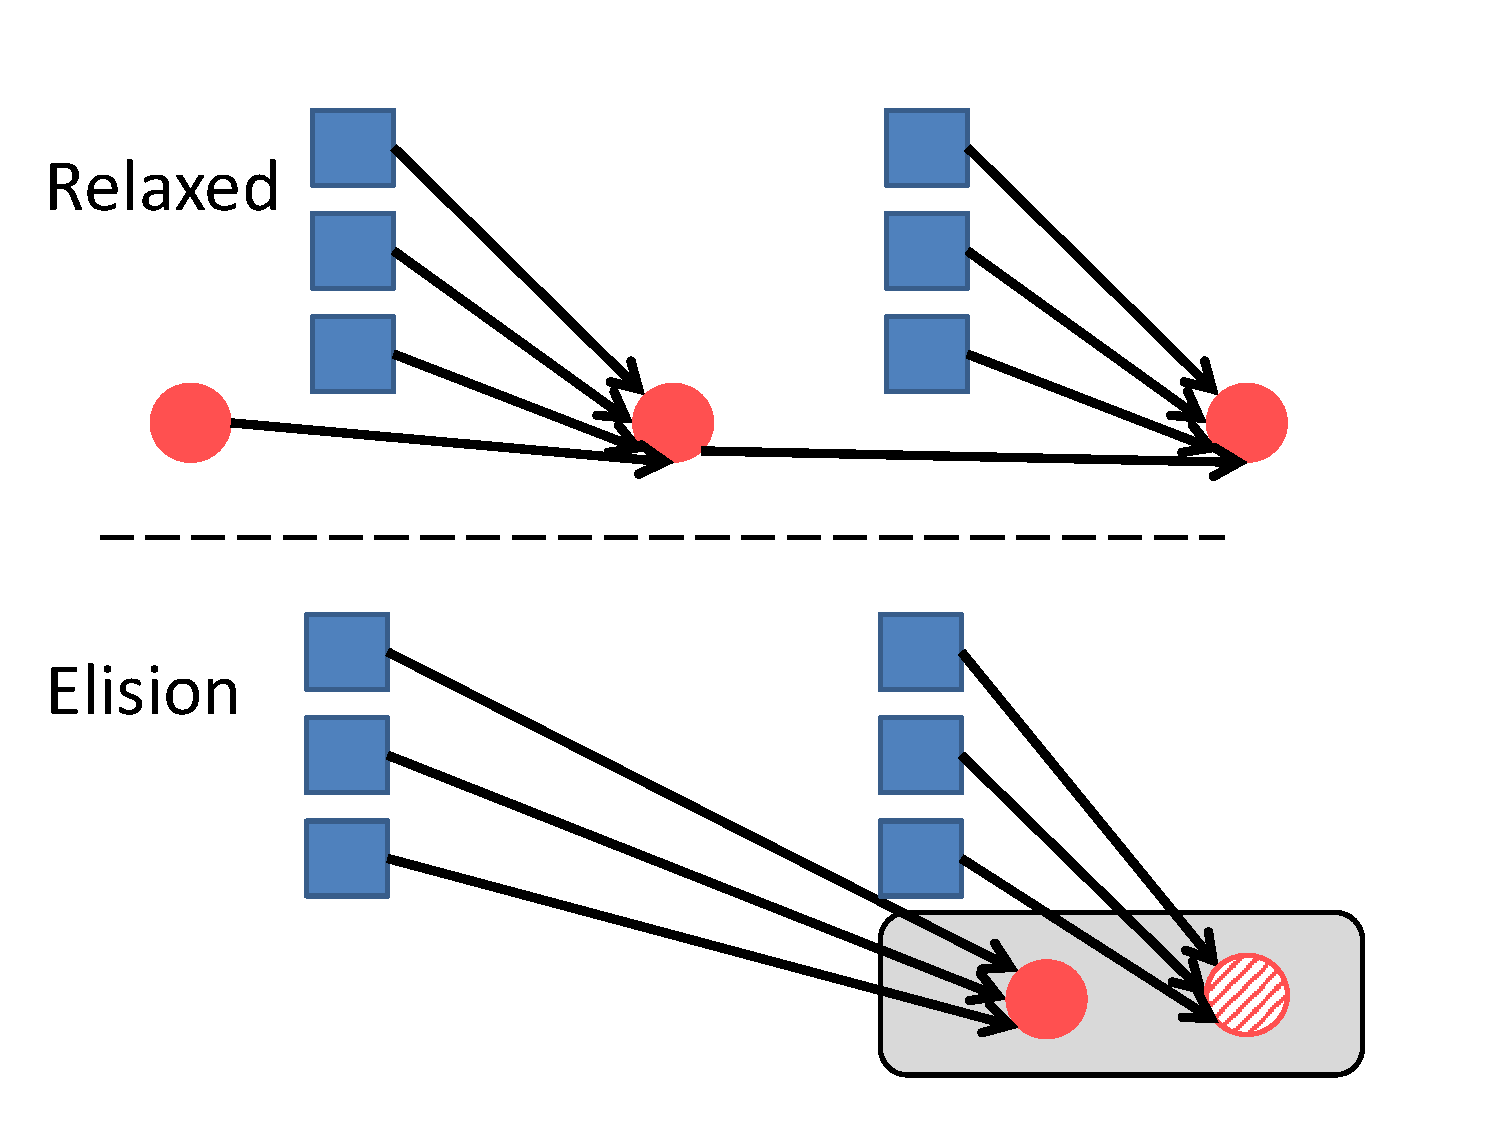
\includegraphics[width=.7\textwidth]{PMC_patterns/buffer_relaxed_elision.pdf}
\caption{\textbf{Buffer execution under relaxed persistent consistency.}  Relaxing persistent consistency removes unnecessary cross-thread dependencies (as in LPO), allows epochs to persist in parallel (as in PEO), and removes unnecessary serial epoch dependencies within threads (top).  Epochs/dependencies are elided by persisting only select counter values (bottom).}
\label{fig:buffer_relaxed_elision}
\end{figure}


I first discuss a persistent buffer, used as an OLTP database centralized log in \fixme{cite}.
This log buffer contains a persistent data array as well as a persistent counter, marking the end of the valid, persistent region of the buffer, shown at the top of Figure~\fixme{ref}.
For simplicity, I neglect details that require data to wrap around the end of the buffer and instead pretend that the valid region of the buffer is always from the base offset of the buffer through the address marked by the counter.
Data are inserted into this buffer by aquiring a volatile lock on the structure, reading the counter to determine the next available address, persisting data to that address, and incrementing the counter by the size of the inserted data before releasing the lock.
For correctness, buffer data must persist before the new counter value persists, and all counter values must persist in order.
These dependencies guarantee that on recovery the valid portion of the buffer will be from the offset through the address marked by the persistent counter.
\fixme{cite} assume the BPFS consistency model, noting that updates to the counter field will cause each thread to stall while the previous value persists.
Instead of considering other hardware and programming interfaces, they provide additional software complexity to allow only intermediate values of the counter to persist.
I believe that their software has a recovery bug in it, but leverage the idea of only persisting intermediate values later.
Additionally, they incorrectly assume that buffer data will persist in parallel.
According to the BPFS model all data dependencies between epochs, even dependencies to volatile data, impose an epoch order, serializing those epochs.

\textbf{PSC.} Under PSC (recall, persistent sequential consistency) all persists to the buffer and counter form a dependence chain, shown at the bottom of Figure~\fixme{ref}.
Every atomically persistable segment of buffer data persists in serial, followed by the new value of the counter.
The next thread to insert into the buffer reads the counter, a shared variable, ordering all subsequent persists after persists of the previous insert.
Assuming log entries are 100 bytes on average, each insert requires 14 serial persists (13 to persist the log entry data, 1 to persist the counter).
If NVRAM persists take even 100ns (a conservative estimate), entries can only be inserted every 1.4\textmu s, on average (any faster and buffers will fill).
This is significantly slower than the throughput of modern concurrent buffers, where cache invalidations take anywhere from 10s to 100s ns (multi-core to multi-socket, respectively).
Without relaxed persistent memory consistency models, NVRAM persists will necessarily create a throughput bottleneck.

\textbf{LPO.} Next I consider the relaxed persistent consistency models introduced in Section~\fixme{ref}, starting with LPO.
Recall that LPO (local persist order) enforcing program-order persist order within threads, but cross-thread dependencies do not enforce persist order without barriers.
Figure~\fixme{ref} shows execution of LPO at the top.
Buffer persists continue to serialize and must persist before the counter, but there is no longer a dependence between the counter persisting and later buffer persists from other threads.
Counter values must still persist in-order, which must be enforced with a persist barrier.
Dependencies \emph{do} exist between counter persists and subsequent buffer persists on the same thread, shown as a dashed line in the Figure.
If every log entry is inserted by a separate thread, LPO results in a persist critical path that involves only counter persists.
However, log entries within a single thread must persist in-order, limiting the throughput of each individual thread.
LPO is easy to program, as all persists within a thread occur-in order, and provides high throughput given sufficient buffering and a large number of threads to yield persist parallelism.

\textbf{TEO.} The bottom of Figure~\fixme{ref} displays buffer execution for TEO -- total epoch order.
Total epoch order allows single-thread persists to occur in parallel by placing them in epochs.
Epochs across threads are ordered (or considered concurrent) according to the consistency model and memory sharing.
By using epochs, TEO allows buffer data to persist in parallel, but still orders buffer persists with counter persists, and counter persists to subsequent buffer persists.
The persist critical path forms a chain of two persist epochs per insert.
Using our earlier assumptions, this buffer will allow inserts every 200ns on average.
While getting closer to the performance of modern volatile concurrent systems, this is still likely slower, and true NVRAM devices may require more than 100ns per serialized persist.
Furthermore, TEO requires frequent persist barriers.
While these epoch barriers are deemed intuitive, they are not as easy to use as sequential consistency (no barriers required) and are more complicated to reason about with multi-threading (as evident by BPFS allowing deadlocks).

\textbf{Relaxed persistent consistency.}
Finally, I imagine a relaxed consistency model for this buffer, shown in Figure~\fixme{ref} (top).
I will not describe the semantics of this model, but rather the dependencies I want it to have.
Like TEO buffer data persists in parallel.
Like LPO there are no dependencies between counter persists subsequent buffer persists.
In fact, this is true even for single-threaded use.
Doing so requires more complicated barriers that do not impose serial dependencies between epochs, but instead allow precise, possibly named dependencies.
For example, a barrier may enforce that a given epoch depends \emph{only} on the following epoch, and no other epochs regardless of thread communication or data dependencies.
Such a barrier would allow a programmer to persist buffer data and guarantee that buffer persists never serialize on counter persists other than the corresponding counter update.

I introduce a final optimization, leveraging \fixme{cite IBM}'s insight that not all values must persist.
Persistent memory consistency models describe the set of \emph{allowable} persistent states, yet not every allowable state must exist in time.
Since the counter is of an atomically persistable size (8 bytes or less), the memory system may defer persisting new values of the counter.
Once the buffer data for two (or more) adjacent log entries successfully persist, the counter value for the last entry persists, implicitly persisting all intermediate counter values at once and validating the log entries.
By recognizing that the counter variable is atomically persistable and exists in an epoch by itself, we might imagine a new epoch barrier that restricts the epoch to a single persist of atomic persist size.
This persist will defer, hoping to coalesce with similar persist epochs.
A new value will eventually persist, but may skip any intermediate values so long as all the coalesced persist epochs' dependencies are satisfied.
The result is that the persist critical path is now bounded to a constant -- persists should never limit the throughput of this buffer (assuming large but finite buffers).

More generally, persist dependencies form a schedule or DAG.
Any nodes in a DAG may be combined into a super node so long as 1) all persists in the super node fit in an atomically persistable size, 2) combining nodes retains the DAG (no cycles), and 3) the super node inherits all dependencies of its member nodes, and all nodes that previously depended on the super node's member nodes now depend on the super node.
An interesting prospect is that as NVRAM technologies progress that atomically persistable size may increase (say, from 8 bytes to 64 bytes).
Larger atomic persists may eventually allow more persist epochs to coalesce into super nodes, decreasing persist critical path, possibly without intervention from the user.
It remains unclear if this property should be leveraged by hardware or in the consistency model, if at all.

\section{Persistent Linked List}
\label{sec:PMC_patterns:LinkedList}

\begin{figure}
\centering
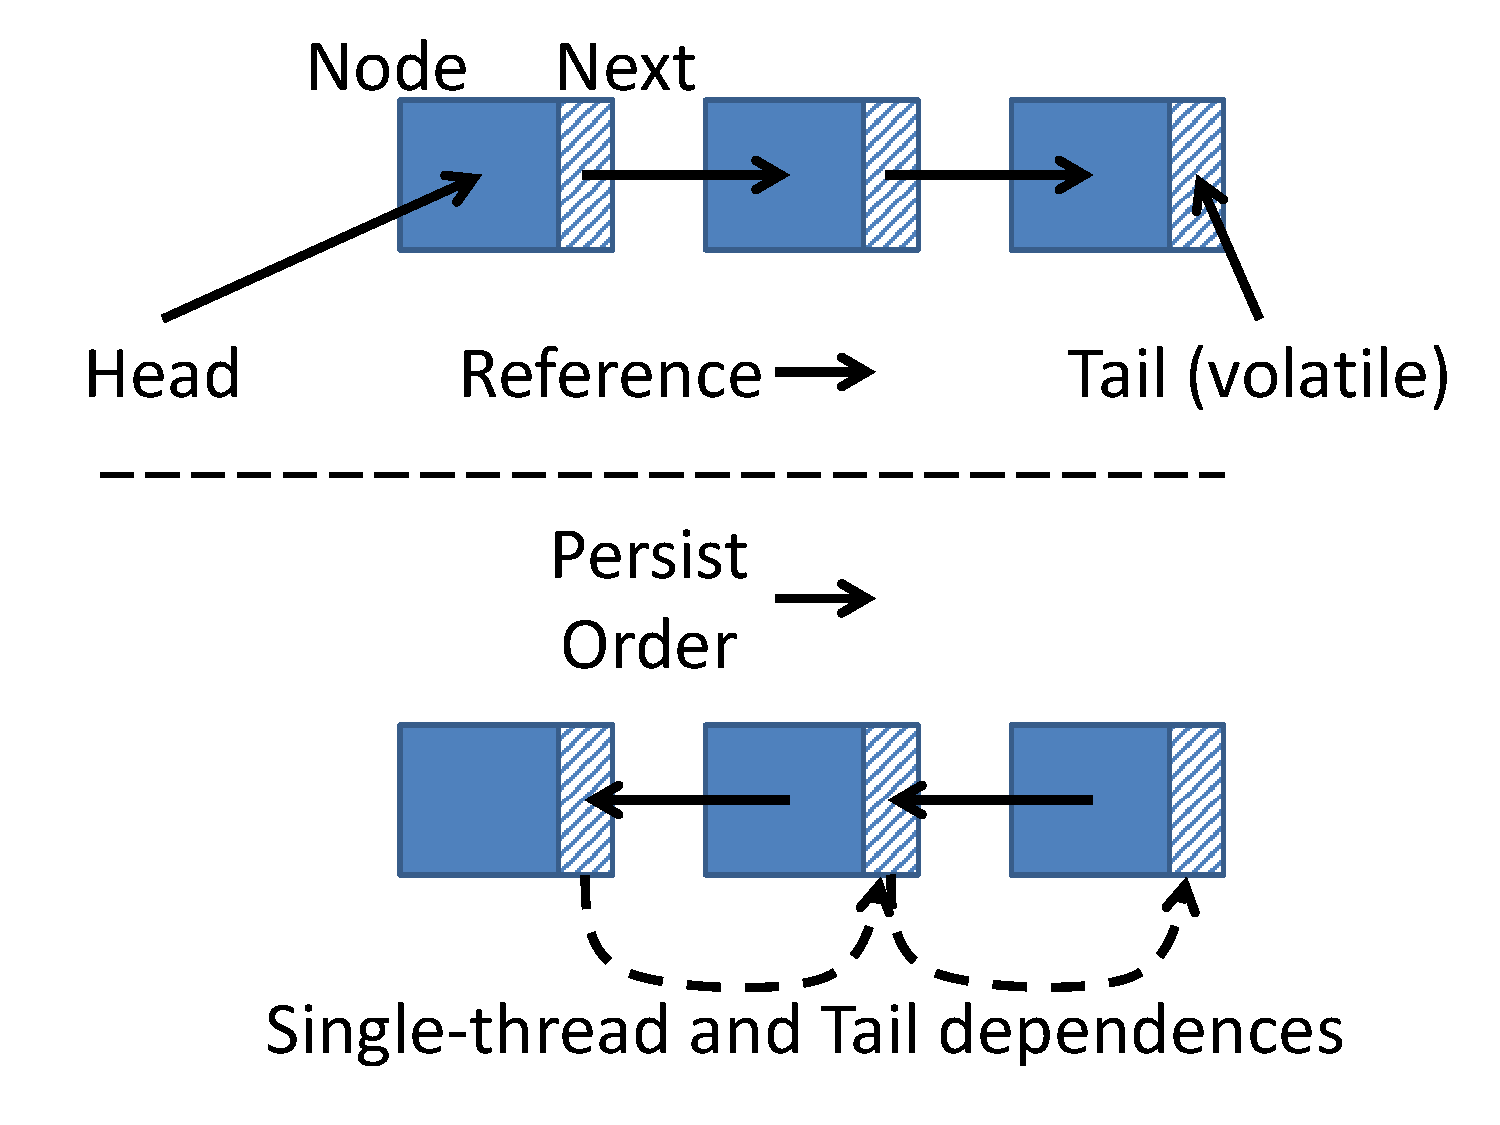
\includegraphics[width=.7\textwidth]{PMC_patterns/linkedlist.pdf}
\caption{\textbf{Persistent linked list.}  The linked list constains nonvolatile Head pointer, volatile Tail pointer, and nodes (data -- solid square; \emph{next} reference -- patterned box).  Nodes persist in parallel (data must still persist before references).  Dashed lines show unnecessary dependencies enforced by strict persistent consistency models, forming a dependence chain.  The valid list is determined at recovery by traversing from Head to the last valid node reference.  Implementing efficient sync remains a challenging.}
\label{fig:LinkedList}
\end{figure}


Finally, I consider a persistent linked list, shown in Figure~\fixme{ref}.
The linked list contains a persistent Head reference, persistent nodes (each containing a \emph{next} reference), and a volatile Tail reference to quickly find the end of the list for insertion (although we assume that at recovery the list will only be traversed from the Head).
Unlike the persistent buffer, where log entries could persist in parallel and the counter was overwritten, the linked list does not overwrite any values as new nodes are added.
For correctness, node data must persist before node \emph{next} references.
However, strict persistent consistency models will enforce that all nodes persist in the order that they are inserted into the list (shown as dotted lines in the bottom of the Figure).
Ignoring sync operations briefly, it would be correct to allow nodes to persist in parallel (reference persists still ordered after data), and simply determine the persistent and valid portion of the list at recovery.
Doing so bounds the persist critical path to a constant.
However, there is now no efficient way to sync the list short of traversing the entire list again, ordering the sync after all persists within the traversal.
This is an interesting design for persistent lists that require high throughput, rarely sync, and prefer linked lists (perhaps to insert in the middle).
Faster, more efficient, yet intuitive sync design remains an interesting challenge.

\section{Conclusion and Future Work}
\label{sec:PMC_patterns:Conclusion}

This chapter considered persistent memory consistency from a performance perspective.
I investigated two simple programming patterns, considering how my proposed persistent consistency models might perform and considering additional optimizations, separate from consistency models, necessary to increase persistent data structure throughput.

For the future, I would like to develop these ideas and form some sort of methodology to support that persistent memory consistency models are a necessary tool and require further investigation.
To start, I would like to implement the above data structures, annotating the code with persist dependencies and using a timing model similar to the one outlined in Section~\fixme{ref}.
Additionally, I would consider implementing these models in Shore-MT.
Finally, I will consider additional models if these do not provide sufficient performance, or I discover that other models provide enough performance and are easier to program for.
I am attempting to submit a paper to this upcoming ISCA, November 2013, and defend next year (2014).

Future work (hopefully outside the scope of my thesis) might consider an evaluation framework that does not require code annotation -- programs are written truly assuming the consistency models.
Additionally, future work will consider actual hardware implementations of useful persistent memory consistency models.
